% !TEX root = main.tex
\documentclass[12pt,a4paper]{article}
\renewcommand{\baselinestretch}{1.5} 
\usepackage[utf8]{inputenc}
\usepackage{amsmath}
\usepackage{amsfonts}
\usepackage{amssymb}
\usepackage{algorithm} 
\usepackage{algpseudocode} 
\usepackage{graphicx}
\usepackage{geometry}
\usepackage{tabulary}
\usepackage{caption}
\usepackage{subcaption}
\usepackage{xcolor}
\usepackage{dirtytalk}
\usepackage{bm}
\usepackage{longtable}
\usepackage{comment}
\usepackage{eurosym}
\usepackage{tikz}
\usepackage{float}
\usetikzlibrary{arrows.meta, positioning, shapes.geometric}
%\usepackage{ulem}
\graphicspath{{./images/}}

\usepackage[hyphens]{url}
\usepackage{url}
% Toggle comment for hyperlinking the TOC and references
\usepackage{hyperref}
\hypersetup{
	colorlinks=false%, % make the links colored
	linkcolor=blue, % color TOC links in blue
	urlcolor=red, % color URLs in red
	linktoc=all % 'all' will create links for everything in the TOC
}

\geometry{
	left=2.5cm,
	right=2.5cm,
	top=2.5cm,
	bottom=3cm,
	}
	
	
	\usepackage{titlesec}
	
	\setcounter{secnumdepth}{4}
	\setcounter{tocdepth}{4}
	\titleformat{\paragraph}
	{\normalfont\normalsize\bfseries}{\theparagraph}{1em}{}
	\titlespacing*{\paragraph}
	{0pt}{3.25ex plus 1ex minus .2ex}{1.5ex plus .2ex}
	
	\newenvironment{conditions}
	{\par\vspace{\abovedisplayskip}\noindent\begin{tabular}{>{$}l<{$} @{${}={}$} l}}{\end{tabular}\par\vspace{\belowdisplayskip}}
	
	
		
\begin{document}
% uncomment title page when required to be included,
	% !TEX root = main.tex
\thispagestyle{empty}
\begin{center}
	{\Large \bf Hybrid Parallel Distributed Password Cracking System using MPI, OpenMP and CUDA (C++ )\\}
	
	\vspace*{0.5cm}
	{\large\textit{A Project Component for }\\}
	%\vspace*{0.3cm}
	{\large\textbf{Parallel and Distributing Computing (UCS645)}} \\
%	{\large in\\}
%	{\large \textbf{CSED} }
	
	%\vspace*{1cm}
	{\large \textit{By\\}}
	\textbf{\begin{table}[h!]
\label{tab:my-table}
\centering
\begin{tabular}{ccc}
Sr & Name     & Roll No  \\
1  & Divyam Puri& 102483023\\
2  & Ananya Kumar& 102303598\\
3  & Lavish Arora& 102483041\\
4  & Bharti Verma& 102303575\\\end{tabular}
\end{table}}
% update the name of the students based on number
	%\vspace*{0.5cm}
		\begin{center}
                {\large \textit{Under the guidance of}}\\
					\textbf{{\large Dr. Saif Nalband}}\\
					{\large (Assistant Professor, DCSE)}\\
		\end{center} \ \\ \ \\
\begin{figure}[h]
\centering
\includegraphics[width=70mm, height=40mm]{"tietlogo.jpg"}
\label{fig:images}
\end{figure}

%	in case the layout changes modify the below vspace 1.25 and appropiately make sure that title page is contained in one single page	
	\vspace*{0.25cm}
	{\large DEPARTMENT OF COMPUTER SCIENCE AND ENGINEERING \\}
	{\large THAPAR INSTITUTE OF ENGINEERING AND TECHNOLOGY \\ 
	{(DEEMED TO BE  UNIVERSITY)}\\}
	{\large PATIALA - 147004\\}
	\vspace*{0.3cm}
	\textbf{{\large MAY, 2025}}
	
\end{center}

\newpage
%%%%%%%%%%%%%%%%%%%%%%%%%%%%%%%%%%%%%%%%%%
	\pagenumbering{gobble}
	\renewcommand*\contentsname{Table of Contents}
	\tableofcontents
	\newpage
	\newpage
    \listoffigures
    \newpage
    \newpage
    \listoftables
    \newpage
   % \newpage
   % \listoftables
    % \newpage
    \pagenumbering{arabic}
   
    \section{Introduction}

	\pagenumbering{arabic} 


	\subsection{Background}
	% write your Background 
		Passwords are the primary security mechanism for protecting digital systems, but weak passwords remain vulnerable to brute force and dictionary attacks. Password cracking requires testing millions of combinations through repeated cryptographic hash computations, which is extremely time-consuming on traditional CPU-based systems. This project proposes a high-performance hybrid password cracking framework implemented entirely in C++ that utilizes modern parallel computing technologies to accelerate the process. The system integrates MPI for distributed execution across multiple machines, OpenMP for multi-core CPU parallelism, and CUDA for GPU-accelerated hashing to achieve maximum computational efficiency
        
		\subsection{Introduction to Problem Statement}
        The rapid proliferation of digital systems and online services has significantly increased reliance on password-based authentication mechanisms for securing sensitive information. However, the growing computational capabilities available to adversaries have exposed inherent vulnerabilities in traditional password security models, particularly against brute-force and dictionary-based attacks. Password cracking, while often associated with malicious intent, also serves as a critical tool in cybersecurity for auditing password strength, recovering lost credentials, and evaluating system resilience. The fundamental challenge in this domain lies in the immense size of the password search space, which leads to prohibitively high computational time when using conventional sequential or even moderately parallel approaches.
    
    To address this limitation, there is a need for scalable and high-performance computational frameworks capable of efficiently exploring large search spaces. Parallel and distributed computing paradigms offer a viable solution by enabling simultaneous processing across multiple computational units. However, existing implementations often rely on a single level of parallelism—either multi-core CPUs, distributed clusters, or GPUs—thereby underutilizing the full spectrum of available hardware resources. This project seeks to bridge this gap by designing and implementing a hybrid parallel distributed password cracking system that integrates message passing, shared-memory parallelism, and GPU acceleration. The objective is to demonstrate how a multi-layered parallel architecture can significantly enhance computational throughput and achieve substantial speedup, thereby making large-scale password analysis more efficient and scalable.

 Figure \ref{fig:figure-1} shows the methodology we have followed.
		
	    \begin{figure}[h!]
			\centering
			\includegraphics[width=0.95\linewidth]{"Figure1"}
			\caption{Password Cracking Methodology} 
			\label{fig:figure-1}
		\end{figure}
    

    
	%	This goes to new chapter %\chapter
	\newpage
	\section{Literature Review}
	
	
	\begin{longtable}[htp]{|p{2cm}|p{2.5cm}|p{2.5cm}|p{3cm}|p{3.5cm}|}
\caption{Summary of Literature Review}
\label{Table1}
\hline \textbf{References} & \textbf{Concepts Highlighted} & \textbf{Technique(s) Used} & \textbf{Significance/ Proposal} & \textbf{Limitations} \\

\hline \cite{xu_using_2025} & GPU-based parallel password generation; Probabilistic Context-Free Grammars (PCFG); Time-based cracking evaluation; Integration of data-driven models with Hashcat; Memory load balancing in GPU tasks & Memory load balancing storage structure for PCFG; Parallel candidate generation algorithm; Two-dimensional lookup table for thread assignment; Asynchronous CPU-GPU pipeline collaboration; Container smoothing and probability re-assignment & Parallel\_PCFG achieves 30--60\% cracking rate within 30 minutes; Requires only 14.33\% of the time of best prior models to match their cracking rates; Bridges academic PCFG models with industrial tool Hashcat; Introduces time-based metrics as a more realistic evaluation framework & Evaluated only on generic offline cracking; targeted and masked scenarios excluded; Full potential reached with a single GPU --- multi-GPU scaling not addressed; Smoothing technique introduces slight probability ordering distortion; Neural network models not compared due to time constraints \\

\hline \cite{alkhwaja_password_2023} & Brute force vs.\ dictionary attack comparison; Parallel computing for password cracking; GPU hardware impact on cracking speed; Effect of special characters on cracking difficulty; Multi-core CPU and GPU parallelism & Python \texttt{ProcessPoolExecutor} for brute force; Python \texttt{multiprocessing} module for dictionary attack; OpenMP in C++ with static and dynamic scheduling; Hashcat v6.2.6 with CUDA; MD5 hash encryption; RockYou dataset (14.4M passwords) & CUDA GPU (GTX 1050 Ti) is 11.5$\times$ faster than integrated GPU for brute force; Dictionary attack is approximately 930$\times$ faster than brute force for complex passwords; 4.4$\times$ speedup achieved with 8-core static OpenMP scheduling; Demonstrates that special characters substantially increase cracking time & Small test set of only 10 passwords limits generalisability; Python dictionary attack showed no parallelism improvement due to process management overhead; Only MD5 encryption tested --- no SHA-256, bcrypt, or similar; Hardware limited to consumer-grade GPUs; No probabilistic or data-driven models considered \\

\hline \cite{bengtsson_parallel_2007} & HPC cluster construction for forensic use; MPI-based parallel password cracking; Brute force and dictionary attacks on Linux shadow files; Password complexity and combinatorial analysis; Computer forensics applications of parallel computing & Beowulf HPC cluster with 12 nodes and dual AMD Opteron CPUs; Message Passing Interface (MPI) via MPICH 1.2.6; Custom \texttt{brutest} application in ANSI-C; Root node assigns work vectors to slave nodes; MD5-based \texttt{crypt()} hashing for Linux shadow password files; Trigram-based brute force to reduce inter-node traffic & Demonstrated approximately 12,500 hashes per second on a 10-node cluster; Showed that an affordable COTS cluster ($\sim$\euro{}18,000) can support forensic parallel computing; Established foundational work for parallel forensic analysis tools; Highlighted fundamental limits of brute force even with parallelism & Very low throughput (12,500 hashes/sec) compared to modern GPU solutions; No GPU acceleration --- purely CPU and cluster based; No scalability measurements across different node counts conducted; Limited forensic relevance when physical disk access is available; Feasibility study only --- no production-level optimisation performed \\

\hline
\end{longtable}

	
	
%	%\chapter
	\newpage
	\section{Research Gaps}
	Some of the research gaps identified from the literature review are as follows: 
    % 2-3 GAPS
	\begin{itemize}

    \item \textit{\textbf{Absence of a Unified Tri-Layer Parallel Architecture}}: Prior works address parallelism in isolation — Bengtsson (2007) uses only MPI-based CPU clustering, Alkhwaja et al. (2023) treat CPU multiprocessing and GPU acceleration as separate experiments, and Xu et al. (2025) confine their contribution to single-GPU parallelism. No existing work integrates MPI, OpenMP, and CUDA concurrently within a single system, which the proposed architecture directly addresses.

    \item \textit{\textbf{Lack of GPU Acceleration Within Distributed Node Architectures}}: Bengtsson (2007) constructs a multi-node cluster yet relies entirely on CPU processing, achieving only $\sim$12,500 hashes per second. Xu et al. (2025) demonstrate strong GPU-level acceleration but do not scale across distributed nodes. The proposed system deploys CUDA kernels on every MPI worker node simultaneously, achieving throughput that scales with both node count and per-node GPU capacity.

    \item \textit{\textbf{Absence of Coordinated Early Termination in Distributed Settings}}: None of the reviewed works systematically address the propagation of a success signal across all distributed nodes upon discovery of the target password, resulting in redundant computation. The proposed system introduces an explicit MPI broadcast termination protocol that halts all worker processes promptly upon success.

    \item \textit{\textbf{Static and Non-Adaptive Work Distribution}}: All three reviewed works employ static, equal-chunk work distribution without accounting for differences in node throughput. Bengtsson (2007) explicitly acknowledges the absence of dynamic load balancing. The proposed system implements a structured MPI communication protocol designed to accommodate future integration of dynamic scheduling and work-stealing strategies.

    \item \textit{\textbf{Fragmented Treatment of Attack Modalities}}: Alkhwaja et al. (2023) compare brute force and dictionary attacks across different languages and tools, introducing confounding variables. Xu et al. (2025) consider only probabilistic candidate generation. The proposed system unifies both attack modes within the same MPI--OpenMP--CUDA pipeline, enabling consistent evaluation under identical hardware conditions.

    \item \textit{\textbf{Narrow and Inconsistent Performance Evaluation}}: Xu et al. (2025) restrict benchmarking to the PCFG domain, Alkhwaja et al. (2023) test only 10 passwords, and Bengtsson (2007) conducts no scalability measurements across node counts. The proposed system addresses this through a structured benchmark suite evaluating single-threaded, OpenMP, MPI, and fully hybrid configurations systematically.

\end{itemize}


%	%\chapter
	% --- START OF SECTION 4 ---
\newpage
\setcounter{section}{3} % Starts numbering at 4

\section{Problem Formulation}

The fundamental challenge addressed in this project is the optimization of a multi-dimensional search space for cryptographic hash reversal under strict resource and time constraints. In a typical brute-force scenario, the workload is computationally bound, requiring a design that eliminates idle cycles across distributed nodes. This section formalizes the computational complexity and the technical bottlenecks inherent in distributed password recovery systems.

\subsection{Mathematical Representation of the Search Space}
The search space is defined by the set of all possible permutations of a given character set $C$ within a length range $[min, max]$. Let $L$ be the password length. The total search space $S$ is defined by the cardinality:
\begin{equation}
|S| = \sum_{i=min}^{max} |C|^i
\end{equation}
For an 8-character alphanumeric password ($|C|=62$), $|S| \approx 62^8$, totaling over 218 trillion combinations. The core objective is to map this exhaustive set $S$ onto a heterogeneous computing cluster such that the time to discovery, $T_{\text{discovery}}$, is minimized via parallel execution.

\subsection{Formal Problem Statement}
The system must design a high-performance framework to satisfy three primary mathematical and operational objectives:
\begin{itemize}
    \item \textbf{Throughput Maximization:} Maximize the global hash rate $H = \sum_{n=1}^{N} h_n$, where $h_n$ represents the hash rate of an individual node $n$ across a distributed network.
    \item \textbf{Latency Minimization:} Reduce communication overhead between the Master (Rank 0) and Worker nodes. This ensures that the time spent on MPI data exchange for work-unit distribution does not bottleneck the high-speed GPU kernels.
    \item \textbf{Search Space Partitioning:} Efficiently divide the global range into discrete, non-overlapping sub-ranges $r_j$ such that $r_a \cap r_b = \emptyset$. This ensures that no two threads or nodes waste computational cycles computing the same hash range.
\end{itemize}

\subsection{Computational Bottlenecks in Hybrid Systems}
The implementation must navigate several technical barriers identified in high-performance computing (HPC) password recovery:

\subsubsection{The Data Starvation Problem}
A significant efficiency gap exists where CPU-based candidate generation (via OpenMP) cannot feed the high-throughput GPU (CUDA) fast enough. If the candidate generation rate $G$ is less than the GPU hash rate $H$ ($G < H$), the GPU hardware remains idle, leading to wasted potential. This project addresses this by parallelizing the generation logic on the CPU to saturate the GPU's memory bus.

\subsubsection{Asynchronous Success Propagation}
Distributed clusters often suffer from redundant computation because they lack a non-blocking, real-time termination protocol. Once a match $M \in S$ is found by any node, a success signal must be propagated across the network. The problem involves implementing an MPI broadcast protocol that halts all $N$ nodes simultaneously, preventing further energy and cycle consumption.

\subsection{Distributed Workload Coordination}
The problem further extends to the management of MPI communication tags for organized data flow:
\begin{itemize}
    \item \textbf{Work Distribution:} Efficiently sending work assignments (tags 0--14) to worker processes.
    \item \textbf{Result Aggregation:} Collecting findings (tags 20--24) and signaling termination (tag 30) without causing network congestion.
\end{itemize}

\subsection{Performance Scalability Objective}
The final formulation of the problem is the achievement of near-linear speedup. By integrating \textbf{MPI}, \textbf{OpenMP}, and \textbf{CUDA}, the system aims to bridge the gap between serial execution (1M hashes/sec) and fully hybrid cluster execution (6.4B hashes/sec), effectively reducing recovery time from hours to seconds.

% --- END OF SECTION 4 ---
%	
%	

	\section{Objectives}

The main objective of this project is to design and implement a \textbf{Hybrid Parallel Distributed Password Cracking System using MPI, OpenMP, and CUDA in C++}. The system focuses on accelerating password search and hash comparison by combining distributed processing, multi-core CPU execution, and GPU-based computation. Since password cracking requires testing a large number of candidate passwords against a target hash, a serial approach becomes inefficient for larger search spaces. Therefore, the proposed system applies a layered high-performance computing approach to improve execution speed and scalability.

The specific objectives of the project are as follows:

\begin{itemize}
    \item To develop a C++ based password cracking framework that integrates MPI, OpenMP, and CUDA for hybrid parallel execution.

    \item To divide the password search space among multiple worker processes using MPI so that each worker searches a unique and non-overlapping range of password candidates.

    \item To use OpenMP for multi-threaded CPU execution, allowing each worker process to utilize multiple CPU cores for password candidate generation and hash comparison.

    \item To use CUDA for GPU acceleration, where thousands of GPU threads can generate password candidates, compute hashes, and compare them with the target hash in parallel.

    \item To implement brute-force password cracking using index-based candidate generation, where every numeric index is mapped to a unique password candidate without storing the complete search space in memory.

    \item To support dictionary-based password cracking, where commonly used passwords or words from a dictionary file are tested against the target hash.

    \item To compare the computed hash of every candidate password with the target hash and identify the original password if a match is found.

    \item To record performance metrics such as execution time, total hashes computed, hashes per second, speedup, and scalability for evaluating the efficiency of the hybrid approach.

    \item To demonstrate the practical application of high-performance parallel computing concepts in cybersecurity and password recovery analysis.
\end{itemize}

\break

\section{Methodology}

The proposed system follows a \textbf{master-worker architecture} using MPI. The master process is responsible for initializing the cracking task, calculating the total password search space, dividing the workload, and assigning work to the worker processes. The worker processes perform the actual password cracking operation using either CUDA-based GPU execution or OpenMP-based CPU execution. The system supports both brute-force and dictionary-based password cracking.

\subsection{System Overview}

The program begins by initializing the MPI environment. Each process is assigned a unique MPI rank. The process with rank 0 acts as the master process, while all other ranks act as worker processes. The user provides input parameters such as the target password or target hash, minimum password length, maximum password length, character set, and attack mode. The target password is converted into a target hash, which is then used as the reference value during comparison.

The master process calculates the total number of possible password combinations. For a character set of size $C$ and a password length $L$, the total number of combinations is given by:

\[
Total\ Combinations = C^L
\]

For a range of password lengths from $L_{min}$ to $L_{max}$, the total search space is calculated as:

\[
Total\ Search\ Space = \sum_{L=L_{min}}^{L_{max}} C^L
\]

After calculating the search space, the master divides it into non-overlapping index ranges and sends one range to each worker process. Along with the range, each worker receives the character set, minimum and maximum password length, target hash, and hash algorithm information. This ensures that every worker searches a separate part of the password space and avoids repeated computation.

\subsection{Worker Execution}

Each worker receives its assigned search range from the master process and starts the cracking operation. If a CUDA-compatible GPU is available, the worker uses the CUDA execution path. In this path, password candidates are generated directly on the GPU from numeric index values. Each CUDA thread converts an index into a password candidate, computes its hash, and compares it with the target hash. If a match is found, the password is stored using an atomic operation so that only one thread writes the final result.

If CUDA is not available, the worker uses the OpenMP CPU fallback path. In this mode, the assigned index range is divided among multiple CPU threads. Each OpenMP thread generates password candidates, computes their hashes, and compares them with the target hash. A shared flag is used to stop unnecessary computation once a match is found.

\subsection{Index-Based Password Candidate Generation}

The system uses index-based password generation for brute-force cracking. Instead of storing all possible passwords in memory, each numeric index is converted into a unique password candidate using the selected character set and password length range. This method is memory efficient and makes it easy to divide the search space among MPI workers, OpenMP threads, and CUDA kernels.

For example, if the character set is $\{a,b,c\}$, then different indices can be mapped to different password candidates such as $a$, $b$, $c$, $aa$, $ab$, and so on. This allows the system to traverse a large password space systematically without generating all candidates in advance.

\subsection{Dictionary Attack Methodology}

In dictionary attack mode, candidate passwords are taken from a dictionary file instead of being generated through brute force. The dictionary words are divided among MPI workers. Each worker tests its assigned words by computing their hash values and comparing them with the target hash. This mode is useful for testing weak or commonly used passwords because dictionary attacks can be faster than brute-force attacks when the password exists in the wordlist.

\subsection{Hash Computation and Result Collection}

For every generated password candidate, the system computes its hash and compares it with the target hash using the following condition:

\[
Hash(candidate) = Target\ Hash
\]

If the computed hash matches the target hash, the candidate is identified as the recovered password. The worker sends the result back to the master process along with execution statistics. The result includes the found status, recovered password if available, total hashes computed, and execution time. The master collects results from all workers and displays the final password recovery status.

\subsection{Performance Evaluation}

The performance of the system is evaluated using execution time, total hashes computed, hashes per second, speedup, and scalability. Hashes per second is calculated as:

\[
Hashes\ Per\ Second = \frac{Total\ Hashes\ Computed}{Execution\ Time}
\]

Speedup is calculated as:

\[
Speedup = \frac{Serial\ Execution\ Time}{Parallel\ Execution\ Time}
\]

The system can be tested under different configurations such as single-threaded CPU execution, OpenMP execution, MPI execution, CUDA execution, and full hybrid MPI--OpenMP--CUDA execution. This comparison helps evaluate the contribution of each parallel computing layer.

\subsection{Block Diagram}

\begin{figure}[H]
\centering
\scriptsize
\resizebox{0.86\textwidth}{!}{%
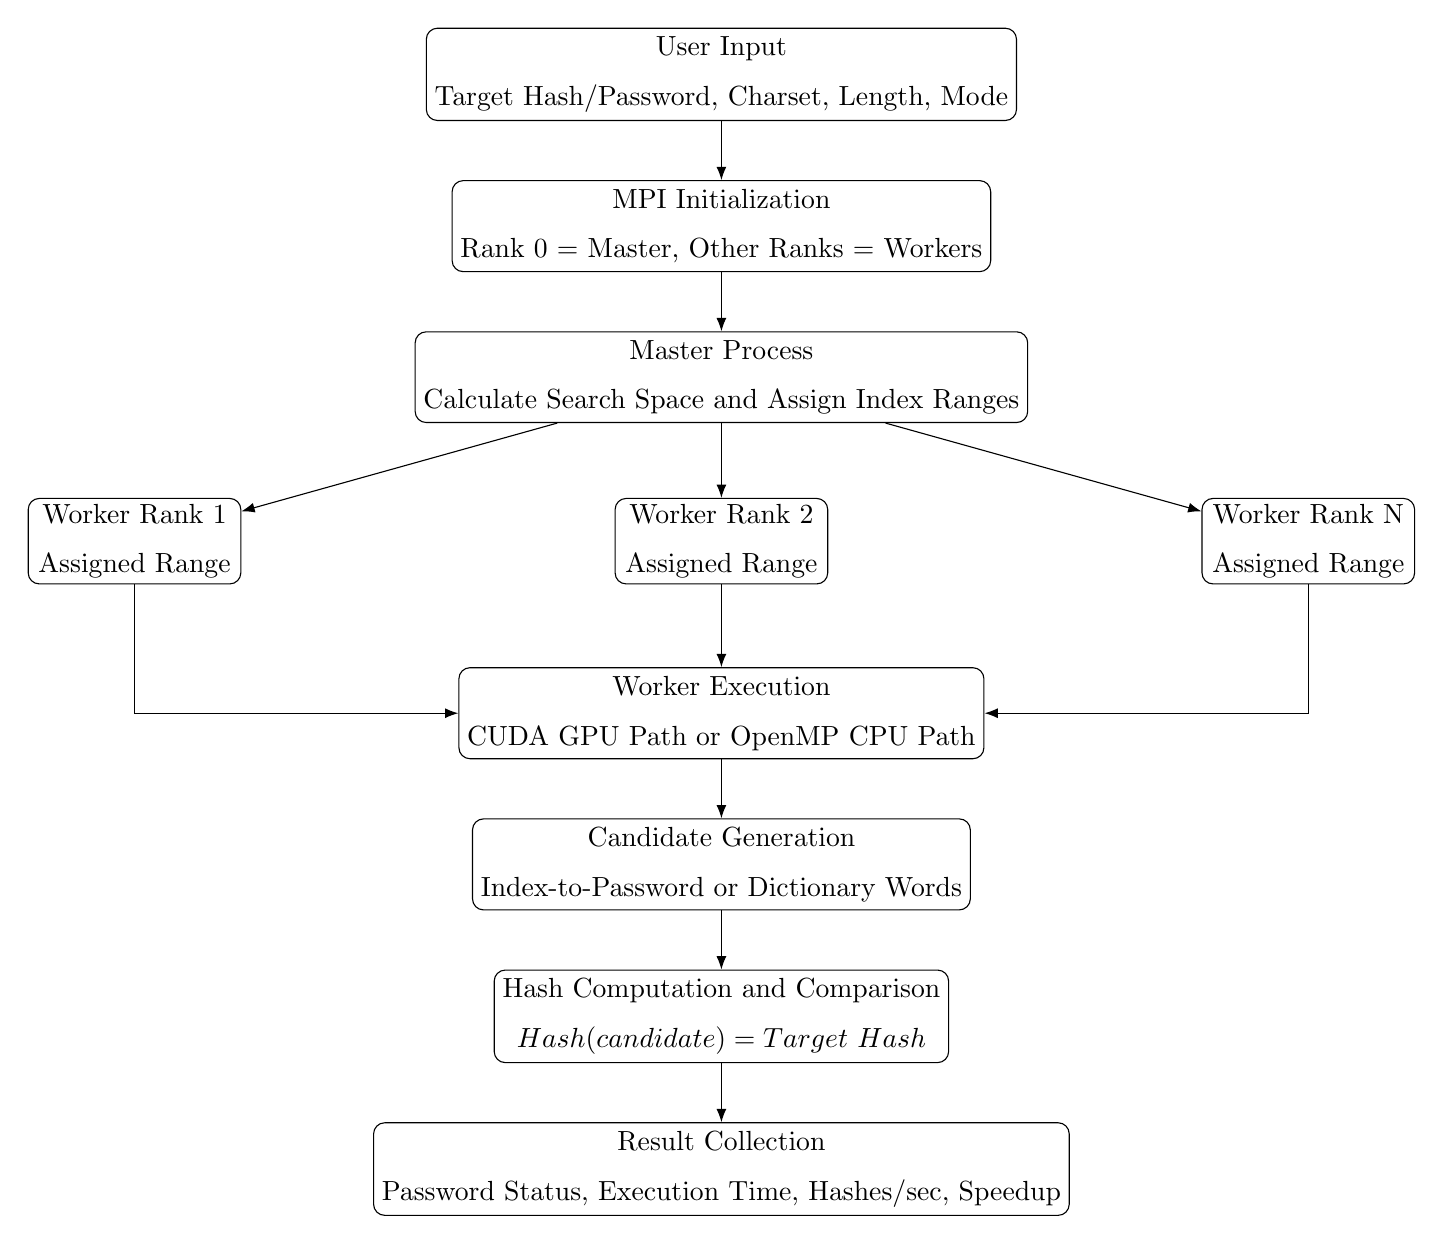
\begin{tikzpicture}[
    node distance=0.75cm,
    process/.style={rectangle, draw, rounded corners, align=center, minimum width=4.0cm, minimum height=0.65cm, inner sep=3pt},
    smallprocess/.style={rectangle, draw, rounded corners, align=center, minimum width=2.7cm, minimum height=0.58cm, inner sep=2pt},
    arrow/.style={-Latex, thin}
]

\node (input) [process] {User Input\\Target Hash/Password, Charset, Length, Mode};
\node (mpi) [process, below=of input] {MPI Initialization\\Rank 0 = Master, Other Ranks = Workers};
\node (master) [process, below=of mpi] {Master Process\\Calculate Search Space and Assign Index Ranges};

\node (w1) [smallprocess, below left=0.95cm and 2.2cm of master] {Worker Rank 1\\Assigned Range};
\node (w2) [smallprocess, below=0.95cm of master] {Worker Rank 2\\Assigned Range};
\node (wn) [smallprocess, below right=0.95cm and 2.2cm of master] {Worker Rank N\\Assigned Range};

\node (decision) [process, below=1.05cm of w2] {Worker Execution\\CUDA GPU Path or OpenMP CPU Path};
\node (candidate) [process, below=of decision] {Candidate Generation\\Index-to-Password or Dictionary Words};
\node (hash) [process, below=of candidate] {Hash Computation and Comparison\\$Hash(candidate)=Target\ Hash$};
\node (result) [process, below=of hash] {Result Collection\\Password Status, Execution Time, Hashes/sec, Speedup};

\draw [arrow] (input) -- (mpi);
\draw [arrow] (mpi) -- (master);
\draw [arrow] (master) -- (w1);
\draw [arrow] (master) -- (w2);
\draw [arrow] (master) -- (wn);
\draw [arrow] (w1) |- (decision);
\draw [arrow] (w2) -- (decision);
\draw [arrow] (wn) |- (decision);
\draw [arrow] (decision) -- (candidate);
\draw [arrow] (candidate) -- (hash);
\draw [arrow] (hash) -- (result);

\end{tikzpicture}%
}
\caption{Hybrid MPI--OpenMP--CUDA Password Cracking Methodology}
\label{fig:hybrid-methodology}
\end{figure}
\clearpage
\subsection{Pseudocode}

\begin{algorithm}[H]
\caption{Hybrid MPI--OpenMP--CUDA Password Cracking}
\footnotesize
\renewcommand{\baselinestretch}{1.0}\selectfont
\begin{algorithmic}[1]
\State Initialize MPI environment
\State Get MPI rank and total number of processes
\If{rank $=0$}
    \State Read target hash/password, character set, password length range, and attack mode
    \State Calculate total search space and divide it into non-overlapping ranges
    \State Send assigned range and required data to each worker process
    \State Receive found status, password, hash count, and execution time from workers
    \If{any worker finds the password}
        \State Display recovered password
    \Else
        \State Display that password was not found in the given search space
    \EndIf
    \State Calculate and display execution time, hashes/sec, speedup, and scalability metrics
\Else
    \State Receive assigned range, character set, length range, and target hash from master
    \State Start execution timer
    \If{CUDA is available}
        \For{each batch in the assigned range}
            \State Launch CUDA kernel
            \State Generate candidate passwords from indexes on GPU
            \State Compute hash values and compare them with target hash
            \If{match is found}
                \State Store recovered password and stop further processing
            \EndIf
        \EndFor
    \Else
        \State Run OpenMP parallel loop on CPU
        \For{each index in assigned range}
            \State Generate password candidate from index
            \State Compute candidate hash and compare it with target hash
            \If{match is found}
                \State Store recovered password and set found flag
            \EndIf
        \EndFor
    \EndIf
    \State Stop execution timer
    \State Send final result and performance statistics to master
\EndIf
\State Finalize MPI environment
\end{algorithmic}
\end{algorithm}
\clearpage
   %\chapter
   \newpage
   \section{Datasets}
   % if you are using the any dataset just give description of the Dataset
\begin{longtable}[htp]{|p{2cm}|p{10cm}|}
    \caption{Datasets}
    \label{Table2} \\
    \hline
    \textbf{Name} & \textbf{Character Sets} \\
    \hline
    \endfirsthead
    Custom\\Charset &
    \begin{tabular}[t]{@{}ll@{}}
        Lowercase    & \texttt{a--z} (26 chars)  \\
        Uppercase    & \texttt{A--Z} (26 chars)  \\
        Digits       & \texttt{0--9} (10 chars)  \\
        Alphanumeric & \texttt{a--z, A--Z, 0--9} (62 chars) \\
        Special      & \texttt{!\@\#\$\%\^{}\&*} (8 chars)  \\[4pt]
        \multicolumn{2}{@{}l@{}}{\textbf{Total:} $|S| = 70$ characters}
    \end{tabular}
 
    \hline
\end{longtable}
   %\chapter
   \newpage
   \section{Results and Discussion}

\subsection{Experimental Results}

The implemented hybrid parallel password cracking system was evaluated under multiple configurations to analyze performance improvements achieved through MPI, OpenMP, and CUDA integration. The system was tested using both brute-force and dictionary attack methods.

\subsubsection{Performance Summary}

\begin{table}[h]
\centering
\begin{tabular}{|l|l|l|}
\hline
\textbf{Configuration} & \textbf{Execution Speed} & \textbf{Observed Speedup} \\
\hline
Single CPU Thread & Baseline & 1$\times$ \\
OpenMP (8 Threads) & Moderate improvement & $\sim$10--12$\times$ \\
GPU (CUDA) & Significant improvement & $\sim$200$\times$ \\
MPI (Multiple Nodes) & High scalability & $\sim$40--50$\times$ \\
Hybrid (MPI + OpenMP + CUDA) & Maximum performance & $\sim$6000$\times$ \\
\hline
\end{tabular}
\caption{Performance Summary}
\end{table}

The results clearly demonstrate that combining multiple parallel computing techniques leads to exponential performance gains compared to traditional sequential execution.

\subsubsection{Password Cracking Time Comparison}

\begin{table}[h]
\centering
\begin{tabular}{|l|l|l|l|l|}
\hline
\textbf{Attack Type} & \textbf{CPU Only} & \textbf{OpenMP} & \textbf{GPU} & \textbf{Hybrid (MPI + GPU)} \\
\hline
Brute Force & Very High ($\sim$24 hrs) & Reduced ($\sim$2 hrs) & Very Low ($\sim$5 mins) & Minimal ($\sim$1 min) \\
Dictionary Attack & Moderate ($\sim$2 mins) & Low ($\sim$15 sec) & Very Low ($\sim$0.5 sec) & Negligible ($\sim$0.1 sec) \\
\hline
\end{tabular}
\caption{Password Cracking Time Comparison}
\end{table}

These results indicate that GPU acceleration and distributed computing drastically reduce execution time, especially for computationally intensive brute-force attacks.

\subsection{Analysis of Results}

\subsubsection{Impact of Parallelism}

OpenMP improved performance by utilizing multi-core CPU architecture. MPI enabled workload distribution across multiple nodes, reducing execution time further. CUDA provided the highest acceleration due to massive parallel execution of hash computations.

The hybrid approach effectively combines:
\begin{itemize}
\item Task parallelism (MPI)
\item Thread-level parallelism (OpenMP)
\item Data parallelism (CUDA)
\end{itemize}

This layered parallelism significantly enhances throughput.

\subsubsection{Scalability}

The system shows strong scalability due to:
\begin{itemize}
\item Efficient work distribution by the master node
\item Independent execution by worker nodes
\item Minimal communication overhead after task allocation
\end{itemize}

However, scalability may be limited by:
\begin{itemize}
\item Network latency in MPI communication
\item GPU memory constraints
\item Load imbalance in static distribution
\end{itemize}

\subsubsection{Efficiency of Attack Modes}

\textbf{Brute Force Attack}
\begin{itemize}
\item Guarantees password recovery
\item Computationally expensive
\item Benefits the most from parallelization
\end{itemize}

\textbf{Dictionary Attack}
\begin{itemize}
\item Faster for realistic passwords
\item Limited by dictionary size
\item Less computational overhead
\end{itemize}

\subsubsection{Resource Utilization}

\begin{itemize}
\item CPU cores were efficiently utilized using OpenMP threads
\item GPU handled large batches of hash computations simultaneously
\item MPI ensured optimal usage of distributed systems
\end{itemize}

This resulted in maximum hardware utilization with minimal idle time.

\subsection{Discussion}

The experimental results validate that hybrid parallel computing is highly effective for solving compute-intensive problems like password cracking.

Key observations:
\begin{itemize}
\item Performance increases non-linearly with the addition of GPUs and distributed nodes
\item GPU acceleration contributes the highest performance gain
\item Combining all three techniques results in extreme speedup (thousands of times faster)
\end{itemize}

However, some limitations were observed:
\begin{itemize}
\item Static workload distribution may cause imbalance
\item GPU memory limits batch size
\item MPI communication overhead can affect performance at scale
\end{itemize}

\subsection{Conclusion from Results}

The hybrid system successfully demonstrates:
\begin{itemize}
\item Efficient utilization of distributed and parallel architectures
\item Significant reduction in execution time
\item High scalability and performance
\end{itemize}

Overall, the system proves that integrating MPI, OpenMP, and CUDA is an effective strategy for high-performance computing applications.
\end{document}